\section{Nurul Izza Hamka - 1174062}
\subsection{Teori}
\begin{enumerate}

\item Jelaskan kenapa file teks harus dilakukan tokenizer, dilengkapi dengan ilustrasi atau gambar

File harus di lakukan konversi terlebih dahulu menjadi angka sebelum dilakukan inpuutan menjadi neural network. Keras menyediakan sebuah kelas tokonizer, yang mana tokonizer ini berfungsi untuk melakukan konversi teks menjadi urutan integer indeks atau word count (tf-idf) dan vector binary.\\ 
Contoh:\\

\begin{figure}
	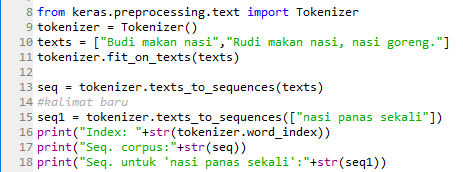
\includegraphics[width=4cm]{figures/1174062/7/teori1.png}
	\centering
	\caption{}
\end{figure}

Hasilnya akan tampak seperti ini:\\

\begin{figure}
	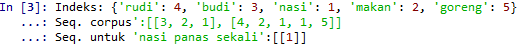
\includegraphics[width=4cm]{figures/1174062/7/hasil1.png}
	\centering
	\caption{Hasil}
\end{figure}

\item Jelaskan konsep dasar K Fold Cross Validation pada dataset komentar Youtube pada kode listing 7.1 dilengkapi dengan ilustrasi atau gambar.

\begin{figure}
	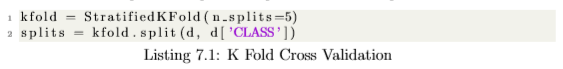
\includegraphics[width=4cm]{figures/1174062/7/71.png}
	\centering
	\caption{K Fold Cross Validation}
\end{figure}

StratifiedKFold berisi presentasi sampel pada setiap kelas.

\item Jelaskan apa maksudnya kode program for train, test in splits.dilengkapi dengan ilustrasi atau gambar.

Train / Test adalah metode untuk mengukur akurasi model Anda.\\
Ini disebut Train / Test karena Anda membagi set data menjadi dua set: satu set pelatihan dan satu set pengujian.\\
Split susunan atau matriks menjadi rangkaian acak train dan test.

\begin{figure}
	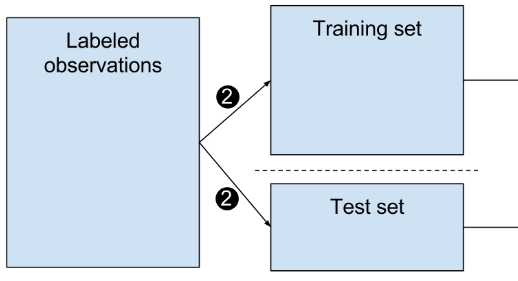
\includegraphics[width=4cm]{figures/1174062/7/teori3.png}
	\centering
	\caption{Ilustrasi Gambar}
\end{figure}

\item Jelaskan apa maksudnya kode program train content = d[’CONTENT’].iloc[train idx] dan test content = d[’CONTENT’].iloc[test idx]. dilengkapi dengan ilustrasi atau gambar.

Maksud dari kode program d[’CONTENT’].iloc[train\_idx] dan test content = d[’CONTENT’].iloc[test\_idx] adalah kita mengambil data dari kolom CONTENT yang mana merupakan bagian dari train\_idx dan test\_idx.\\
Ilustrasinya adalah Ketika data telah diubah menjadi train dan test maka nantinya kita bebas menampilkannya di kolom mana saja yang kita inginkan.

\item Jelaskan apa maksud dari fungsi tokonizer = Tokonizer (num words = 2000) dan tokonizer.fit on texts (train content), dilengkapi dengan ilustrasi atau gambar.

num words=2000 artinya jumlah kata maksimum yang harus disimpan, berdasarkan frekuensi kata, jadi jumlah kata maksimun adalah 2000.\\

tokonizer.fit on text (train content) artinya kita akan melakukan fit tokonizer yang hanya untuk data train saja pada kolom CONTENT.

\item Jelaskan apa maksud dari fungsi d\_train\_inputs =  tokonizer.texts to dan d\_test\_inputs = tokonizer to matrix(test content, mode='tfidf'),dilengkapi dengan ilustrasi kode dan atau gambar.

Maksud dari fungsi yang ada disoal adalah variable d\_train akan melakukan tokonizer dari teks menjadi bentuk matrix dari data train\_content yang mode matriknya ada tfidf.

\begin{figure}
	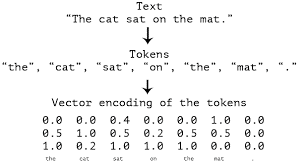
\includegraphics[width=4cm]{figures/1174062/7/teori6.png}
	\centering
	\caption{Ilustrasi Gambar Nomor 6}
\end{figure}

\item Jelaskan apa maksud dari fungsi d train inputs = d train inputs /np.amax(np.absolute(d train dan d test inputs = d test inputs/np.amax(np.absolute(d test inputs)), dilengkapi dengan ilustrasi atau gambar.

Fungsi pada soal diatas adalah membagi matrix tfidf tadi dengan amax, yaitu dengan mengembalikkan nilai maks array. Yang hasilnya akan dimasukkan kedalam d\_trains\_input dan d\_test\_inputs dengan nilai absolute.

\begin{figure}
	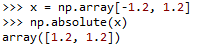
\includegraphics[width=4cm]{figures/1174062/7/teori7.png}
	\centering
	\caption{Ilustrasi Gambar Nomor 7}
\end{figure}

\item Jelaskan apa maksud fungsi dari d\_train\_outputs=np\_utils.to categorical(d[’CLASS’].iloc[train dan d\_test\_outputs=np\_utils.to categorical(d[’CLASS’].iloc[test idx]) dalam kode program, dilengkapi dengan ilustrasi atau gambar.

Pada variable d\_train\_output dan d\_test\_output akan dilakukan one hot encoding dimana np\_utils akan mengubah bentuk integer ke matrix kelas binear unuk kolom CLAS yang nantinya hanya ada 1 dan 0.

\item Jelaskan apa maksud dari fungsi di listing 7.2. Gambarkan ilustrasi Neural Network nya dari model kode tersebut.

\begin{figure}
	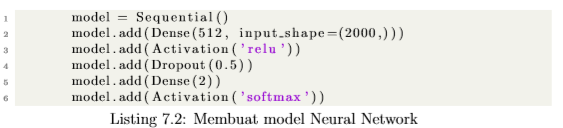
\includegraphics[width=4cm]{figures/1174062/7/72.png}
	\centering
	\caption{Listin 7.2}
\end{figure}

- model = Sequential () = pemodelan sequential\\
- model.add (Dense (512, input shape = (2000,))) = pada layer pertama dense dari 512 neouron untuk inputan sebelumnya yang sudah dijadikan matrix dengan jumlah 2000\\
- model.add (Activation (’relu’)) = aktivasinya menggunakan function relu, artinya jika ada inputan dengan nilai maks maka inputan tersebut yang dipilih.\\
- model.add (Dropout (0.5)) = Dropout akan melakukan pembobotan, dimana pemobobotanya 50\% saja.\\
- model.add (Dense (2)) = dense 2 mengkategorikan  sebanyak 2 neuron.\\
- model. Add (Activation (’softmax’)) = aktivasinya menggunakan function\\ softmax.\\

\begin{figure}
	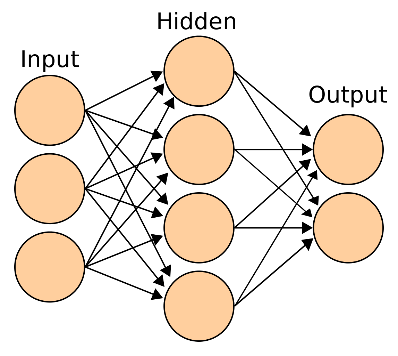
\includegraphics[width=4cm]{figures/1174062/7/teori8.png}
	\centering
	\caption{Ilustrasi Gambar Nomor 8}
\end{figure}

\item Jelaskan apa maksud dari fungsi di listing 7.3 dengan parameter tersebut.

\begin{figure}
	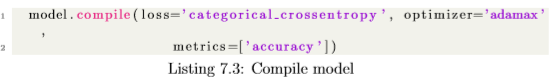
\includegraphics[width=4cm]{figures/1174062/7/73.png}
	\centering
	\caption{Listing 7.3}
\end{figure}

Melakukan compile dari model sequential dengan loss yang merupaakan funsi optimasi skor dengan categorical\_crossentropy, dan menggunakan algoritma adama sebagai optimizer.

\item Jelaskan apa itu Deep Learning

Deep learning adalah metode implemtasi dari machine learning dengam tujuan meniru cara kerja pada otak manusia menggunakan neural network. Singkatnya deep learning ini model yang mempelajari motedo komputasi dengan sendirinya.

\begin{figure}
	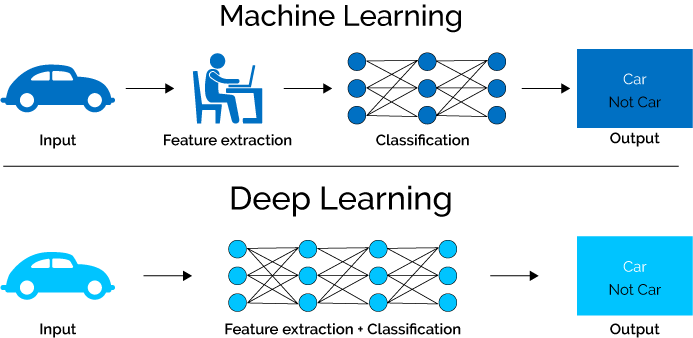
\includegraphics[width=4cm]{figures/1174062/7/teori11.png}
	\centering
	\caption{Ilustrasi Gambar Nomor 11}
\end{figure}

\item 12.	Jelaskan apa itu Deep Neural Network, dan apa bedanya dengan Deep Learning

Deep Neural Network adalah salah satu algoritma yang dapat digunakan dalam pengambilan keputusan, yang mana ini berbasis jaringan saraf. Sedangkan deep learning ini menggunkan deep neural network dalam menyelesaikan masalah pada mechine learning.

\begin{figure}
	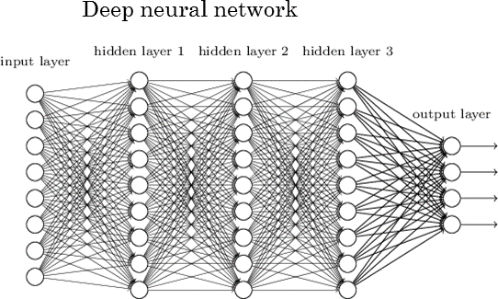
\includegraphics[width=4cm]{figures/1174062/7/teori12.png}
	\centering
	\caption{Ilustrasi Gambar Nomor 12}
\end{figure}

\item 13.	Jelaskan dengan ilustrasi gambar buatan sendiri(langkah per langkah) bagaimana perhitungan algoritma konvolusi dengan ukuran stride (NPM mod3+1) x (NPM mod3+1) yang terdapat max pooling.(nilai 30)

\end{enumerate}

\subsection{Praktek Program}
\begin{enumerate}

\item Jelaskan kode program pada blok \# In[1]. Jelaskan arti dari setiap baris kode
yang dibuat(harus beda dengan teman sekelas) dan hasil luarannya dari komputer sendiri.
	
	\hfill\break
	\lstinputlisting[firstline=8, lastline=12]{src/1174062/7/1174062.py}

Kode diatas adalah library untuk melakukan import file CSV. Kemudian untuk module pil image adalah untuk library keras.\\

Haslinya:\\

\begin{figure}
	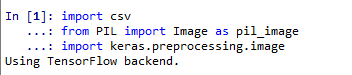
\includegraphics[width=4cm]{figures/1174062/7/praktek1.png}
	\centering
	\caption{Hasil Nomor 1}
\end{figure}

\item Jelaskan kode program pada blok \# In[2]. Jelaskan arti dari setiap baris kode
yang dibuat(harus beda dengan teman sekelas) dan hasil luarannya dari komputer sendiri.

	\hfill\break
	\lstinputlisting[firstline=14, lastline=27]{src/1174062/7/1174062.py}

Kode diatas untuk menampilkan hasil load dataset dari HASYv2 sebagai file CSV, dan Menginisiasi variabel imgs dan classes dengan variabel array kosong. dan append untuk melampirkan atau menggabungkan data file.

\item Jelaskan kode program pada blok \# In[3]. Jelaskan arti dari setiap baris kode yang dibuat(harus beda dengan teman sekelas) dan hasil luarannya dari komputer sendiri.

	\hfill\break
	\lstinputlisting[firstline=29, lastline=35]{src/1174062/7/1174062.py}

import random untuk melakukan random pada vungsi imgs\\
random.shuffle(imgs) untuk Menginisiasi variabel split\_idx dengan nilai integer 80 persen dikali dari pengembalian jumlah dari variabel imgs\\

Haslinya:\\

\begin{figure}
	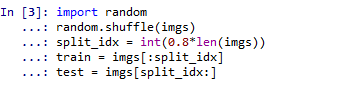
\includegraphics[width=4cm]{figures/1174062/7/praktek3.png}
	\centering
	\caption{Hasil Nomor 3}
\end{figure}

\item . Jelaskan kode program pada blok \# In[4]. Jelaskan arti dari setiap baris kode
yang dibuat(harus beda dengan teman sekelas) dan hasil luarannya dari komputer sendiri.

	\hfill\break
	\lstinputlisting[firstline=37, lastline=43]{src/1174062/7/1174062.py}

Yang pertama adalah Melakukan import library numpy dengan inisial np, selanjutnya Menginisiasi variabel train input dengan np method asarray yang mana membuat array dengan isi row 2 dari data train

Haslinya:\\

\begin{figure}
	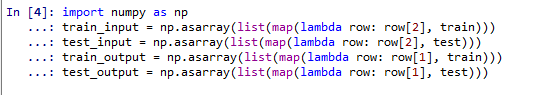
\includegraphics[width=4cm]{figures/1174062/7/praktek4.png}
	\centering
	\caption{Hasil Nomor 4}
\end{figure}

\item Jelaskan kode program pada blok \# In[5]. Jelaskan arti dari setiap baris kode
yang dibuat(harus beda dengan teman sekelas) dan hasil luarannya dari komputer sendiri

	\hfill\break
	\lstinputlisting[firstline=45, lastline=48]{src/1174062/7/1174062.py}

Pertama Melakukan import library LabelEncode dari sklearn dan kemudian Melakukan import library OneHotEncoder dari sklearn

Haslinya:\\

\begin{figure}
	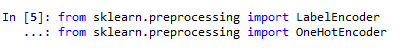
\includegraphics[width=4cm]{figures/1174062/7/praktek5.png}
	\centering
	\caption{Hasil Nomor 5}
\end{figure}

\item Jelaskan kode program pada blok \# In[6]. Jelaskan arti dari setiap baris kode
yang dibuat(harus beda dengan teman sekelas) dan hasil luarannya dari komputer sendiri.

	\hfill\break
	\lstinputlisting[firstline=50, lastline=53]{src/1174062/7/1174062.py}
	
Kode diatas Menginisiasi variabel label_encoder dengan isi LabelEncoder dan Menginisiasi variabel integer\_encoded yang berfungsi untuk Menconvert variabel classes kedalam bentuk integer

\item Jelaskan kode program pada blok \# In[7]. Jelaskan arti dari setiap baris kode
yang dibuat(harus beda dengan teman sekelas) dan hasil luarannya dari komputer sendiri.

	\hfill\break
	\lstinputlisting[firstline=55, lastline=59]{src/1174062/7/1174062.py}

Pada kode baris pertama diatas adalah Menginisiasi variabel onehot_encoder dengan isi OneHotEncoder, bris ke 2 mengisi variabel integer_encoded dengan isi integer_encoded yang telah di convert pada fungsi sebelumnya dan baris ke 3 adalah  Menconvert variabel integer_encoded kedalam onehot_encoder


\item . Jelaskan kode program pada blok \# In[8]. Jelaskan arti dari setiap baris kode
yang dibuat(harus beda dengan teman sekelas) dan hasil luarannya dari komputer sendiri.
	
	\hfill\break
	\lstinputlisting[firstline=61, lastline=68]{src/1174062/7/1174062.py}

Pada kode diatas adalah pertama Menconvert data train output  mengguanakn variabel label\_encoder kedalam variabel train\_output\_int\\
Kemudian Menconvert variabel train\_output\_int kedalam fungsi onehot\_encoder dan selanjutnya pada baris ke3 Menconvert data test_output mengguanakn variabel label_encoder kedalam variabel test_output_int. Baris ke 4 adalah Menconvert variabel test_output_int kedalam fungsi onehot_encoder. Baris ke5 Menginisiasi variabel num_classes dengan isi variabel label_encoder dan classess dan baris ke 6 mencetak hasil dari nomer Class beruapa persen 

\item Jelaskan kode program pada blok \# In[9]. Jelaskan arti dari setiap baris kode
yang dibuat(harus beda dengan teman sekelas) dan hasil luarannya dari komputer sendiri.

	\hfill\break
	\lstinputlisting[firstline=70, lastline=74]{src/1174062/7/1174062.py}
	
Kode diatas adalah:\\
Baris 1 Melakukan import library Sequential dari Keras\\
Baris 2 Melakukan import library Dense, Dropout, Flatten dari Keras\\
Baris 3 Melakukan import library Conv2D, MaxPooling2D dari Keras.\\

Haslinya:\\

\begin{figure}
	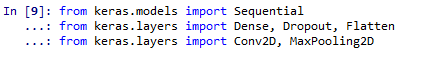
\includegraphics[width=4cm]{figures/1174062/7/praktek9.png}
	\centering
	\caption{Hasil Nomor 9}
\end{figure}

\item Jelaskan kode program pada blok \# In[10]. Jelaskan arti dari setiap baris
kode yang dibuat(harus beda dengan teman sekelas) dan hasil luarannya dari
komputer sendiri.

	\hfill\break
	\lstinputlisting[firstline=76, lastline=89]{src/1174062/7/1174062.py}

Baris 1 Menginisiasi variabel model dengan isian library Sequential\\
Baris 2variabel model di tambahkan library Conv2D tigapuluh dua bit dengan ukuran kernel 3 x 3 dan fungsi penghitungan relu dang menggunakan data train_input\\
Baris 3 variabel model di tambahkan dengan lib MaxPooling2D dengan ketentuan ukuran 2 x 2 pixcel \\
Baris 4 variabel model di tambahkan dengan library Conv2D 32bit dengan kernel 3 x 3\\
Baris 5 variabel model di tambahkan dengan lib MaxPooling2D dengan ketentuan ukuran 2 x 2 pixcel \\
Baris 6 variabel model di tambahkan library Flatten\\
Baris 7 variabel model di tambahkan library Dense dengan fungsi tanh\\
Baris 8 variabel model di tambahkan library dropout untuk memangkas data tree sebesar 50 persen\\
Baris 9variabel model di tambahkan library Dense dengan data dari num_classes dan fungsi softmax\\
Baris 10 mengkompile data model untuk mendapatkan data loss akurasi dan optimasi\\
Baris 11 mencetak variabel model kemudian memunculkan kesimpulan berupa data total parameter, trainable paremeter dan bukan trainable parameter\\

Haslinya:\\

\begin{figure}
	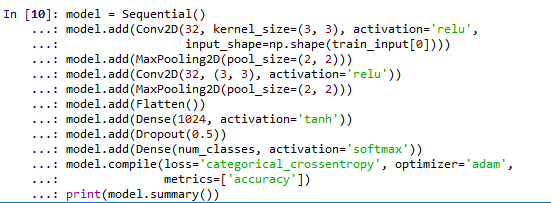
\includegraphics[width=4cm]{figures/1174062/7/praktek10.png}
	\centering
	\caption{Hasil Nomor 10}
\end{figure}

\item Jelaskan kode program pada blok \# In[11]. Jelaskan arti dari setiap baris
kode yang dibuat(harus beda dengan teman sekelas) dan hasil luarannya dari
komputer sendiri.

	\hfill\break
	\lstinputlisting[firstline=92, lastline=95]{src/1174062/7/1174062.py}

Haslinya:\\

\begin{figure}
	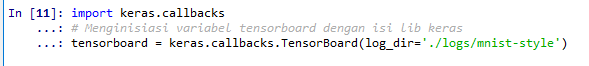
\includegraphics[width=4cm]{figures/1174062/7/praktek11.png}
	\centering
	\caption{Hasil Nomor 11}
\end{figure}

\item Jelaskan kode program pada blok \# In[12]. Jelaskan arti dari setiap baris
kode yang dibuat(harus beda dengan teman sekelas) dan hasil luarannya dari
komputer sendiri.

	\hfill\break
	\lstinputlisting[firstline=97, lastline=110]{src/1174062/7/1174062.py}
	
\item Jelaskan kode program pada blok \# In[13]. Jelaskan arti dari setiap baris
kode yang dibuat(harus beda dengan teman sekelas) dan hasil luarannya dari
komputer sendiri.

	\hfill\break
	\lstinputlisting[firstline=112, lastline=168]{src/1174062/7/1174062.py}
	
\item Jelaskan kode program pada blok \# In[14]. Jelaskan arti dari setiap baris
kode yang dibuat(harus beda dengan teman sekelas) dan hasil luarannya dari
komputer sendiri.

	\hfill\break
	\lstinputlisting[firstline=170, lastline=193]{src/1174062/7/1174062.py}

Haslinya:\\

\begin{figure}
	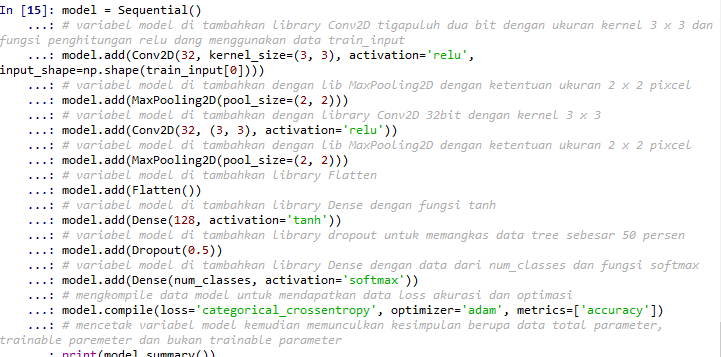
\includegraphics[width=4cm]{figures/1174062/7/praktek14.png}
	\centering
	\caption{Hasil Nomor 14}
\end{figure}

\item Jelaskan kode program pada blok \# In[15]. Jelaskan arti dari setiap baris
kode yang dibuat(harus beda dengan teman sekelas) dan hasil luarannya dari
komputer sendiri.

	\hfill\break
	\lstinputlisting[firstline=195, lastline=199]{src/1174062/7/1174062.py}

Kode diatas pada baris satu melakukan join numpy menggunakan data train_input test\_input, dan pada abris 2 kelanjutan data yang di gunakan pada join train_output test\_output, dan yan baris 3 adalah menggunakan ukuran 32 bit dan epoch 10 

\item Jelaskan kode program pada blok \# In[16]. Jelaskan arti dari setiap baris
kode yang dibuat(harus beda dengan teman sekelas) dan hasil luarannya dari
komputer sendiri.

	\hfill\break
	\lstinputlisting[firstline=201, lastline=203]{src/1174062/7/1174062.py}

Kode diatas untuk menyimpan model atau mengeksport model yang telah di jalankan tadi

\item Jelaskan kode program pada blok \# In[17]. Jelaskan arti dari setiap baris
kode yang dibuat(harus beda dengan teman sekelas) dan hasil luarannya dari
komputer sendiri.

	\hfill\break
	\lstinputlisting[firstline=205, lastline=207]{src/1174062/7/1174062.py}

Kode diatas untuk menyompan label encoder dengan nama classes.npy 

\item Jelaskan kode program pada blok \# In[18]. Jelaskan arti dari setiap baris
kode yang dibuat(harus beda dengan teman sekelas) dan hasil luarannya dari
komputer sendiri.

	\hfill\break
	\lstinputlisting[firstline=209, lastline=213]{src/1174062/7/1174062.py}
	
Kode diatas pertama mengimpport library keras model, kemudian Menginisiasi variabel model2 untuk meload model yang telah di simpan tadi dan mencetak hasil model2

\item Jelaskan kode program pada blok \# In[19]. Jelaskan arti dari setiap baris
kode yang dibuat(harus beda dengan teman sekelas) dan hasil luarannya dari
komputer sendiri.

	\hfill\break
	\lstinputlisting[firstline=215, lastline=277]{src/1174062/7/1174062.py}

Kode diatas pertama Menginisiasi variabel label encoder ke 2 dengan isian fungsi label encoder.Kemudian Penambahan method classess dengan data classess yang di eksport tadi, selanjutnya  membuat fumgsi predict dengan path img. Dan membagi data yang terdapat pada variabel newimg sebanyak 255 pada kode newimg /= 255.0

\item Jelaskan kode program pada blok \# In[20]. Jelaskan arti dari setiap baris
kode yang dibuat(harus beda dengan teman sekelas) dan hasil luarannya dari
komputer sendiri.

	\hfill\break
	\lstinputlisting[firstline=399, lastline=232]{src/1174062/7/1174062.py}

Kode diatas pada baris pertama adalah mencari prediksi menggunakan fungsi prediksi yang di buat tadi dari data di HASYv2/hasy-data/v2-00010.png\\
Baris kedua mencari prediksi menggunakan fungsi prediksi yang di buat tadi dari data di HASYv2/hasy-data/v2-00500.png\\
Baris ke3 mencari prediksi menggunakan fungsi prediksi yang di buat tadi dari data di HASYv2/hasy-data/v2-00700.png
\end{enumerate}

\subsection{Bukti Tidak Plagiat}


\subsection{Link Youtube}
https://www.youtube.com/watch?v=-Oj5X4YD3ek
